\documentclass[9pt,mathserif,aspectratio=169]{beamer}
\usepackage[utf8]{inputenc} %Some citations and accents need this

%\useoutertheme{smoothbars} %Disabled: too many sections causes header overflow
\setbeamertemplate{headline}{} %Clean header -- no navigation bar
\usetheme{Dal_4x3}
\usecolortheme{Dal}

\usepackage{transparent} % \transparent{0.3}{ <stuff> } will make that stuff have 30% opacity.
\usepackage{changepage} % \begin{adjustwidth}{+50pt}{-200pt} will add 50pt to left margin, take 200pt from right

\usepackage{upgreek} %To get \uppi
	\renewcommand{\pi}{\uppi}
	\newcommand{\e}{\mathrm{e}} %Exponential
	\renewcommand{\i}{\mathrm{i}} %Imaginary Number
\usepackage{bm} %Very outdated package that still works for bolding greek letters.
\usepackage{pifont}% For checkmarks and x's
	\newcommand{\cmark}{\ding{51}}%
	\newcommand{\xmark}{\ding{55}}%

\usepackage{tcolorbox}
\usepackage{braket}
\usepackage{bm} %Bold math \bm and \boldsymbol
	\newcommand{\bs}{\boldsymbol}
\usepackage{animate} %Alternate for animations
\usepackage{verbatim}
\usepackage{chemformula} %\ch{H2}
\usepackage{listings}
\usepackage{ragged2e} %For \justifying
\usepackage{physics} %Adds \abs{} for absolute value brackets, and other physics related commands
\usepackage{braket} %Adds \braket{0|0}, \bra{0}, or \ket{0}
\usepackage{ulem}
\usepackage{cancel} %For \cancelto
\usepackage[hang,flushmargin]{footmisc} %To remove indent from footnote
\usepackage{caption, subcaption} %Adds \begin{subfigure}{0.5\textwidth}{} \caption{}... to existing figures.
\usepackage{parskip}
	\setlength{\parskip}{\smallskipamount}
	\setlength{\parindent}{0pt}
\usepackage{appendixnumberbeamer}


\usepackage{amstext} 	% for \text macro
\usepackage{array}	 	% for \newcolumntype macro
\usepackage{booktabs}	% for \toprule \midrule \bottomrule in tables
	\newcolumntype{L}{>{$}l<{$}} % math-mode version of "l" column type
	\newcolumntype{C}{>{$}c<{$}} % math-mode version of "c" column type
	\newcolumntype{R}{>{$}r<{$}} % math-mode version of "r" column type



%%%%%%%%%%%%%%%%%% for \rowcolor
\usepackage{xcolor,colortbl}
%%%%%%%%%%%%%%%%%%


%Write Fortran code with syntax highlighting
\definecolor{snow}{rgb}{1.0, 0.98, 0.98}
\definecolor{lavendergray}{rgb}{0.77, 0.76, 0.82}
\definecolor{charcoal}{rgb}{0.21, 0.27, 0.31}
\definecolor{black}{rgb}{0.0, 0.0, 0.0}
\definecolor{huntergreen}{rgb}{0.21, 0.37, 0.23}
\definecolor{burntorange}{rgb}{0.8, 0.33, 0.0}
\definecolor{darkred}{rgb}{0.55, 0.0, 0.0}
\lstset{
	language=Fortran,
    backgroundcolor=\color{snow},
    numberstyle=\small\color{lavendergray},
    commentstyle=\color{charcoal},
    identifierstyle=\color{black},
    stringstyle=\color{huntergreen},
    keywordstyle=\bfseries\color{burntorange},
    basicstyle=\scriptsize\ttfamily,
    breakatwhitespace=false,
    breaklines=true,
    captionpos=b,
    keepspaces=true,
    numbers=left,
    numbersep=5pt,
    showspaces=false,
    showstringspaces=false,
    showtabs=false,
    tabsize=2
}

%textpos already loaded via documentclass options
\newcommand{\source}[1]{\begin{textblock*}{12cm}(0.5cm,8.5cm)
    \begin{beamercolorbox}[ht=0.2cm,left]{framesource}
        \usebeamerfont{framesource}\usebeamercolor[fg]{framesource} {#1}
    \end{beamercolorbox}
\end{textblock*}}
%\setbeamercolor{framesource}{fg=gray}
\setbeamerfont{framesource}{size=\tiny}


%Uncovering graphics with transparency
\newcommand<>{\uncovergraphics}[2][{}]{
    % Taken from: <https://tex.stackexchange.com/a/354033/95423>
    \begin{tikzpicture}
    \node[anchor=south west,inner sep=0] (B) at (4,0)
        {\includegraphics[#1]{#2}};
    \alt#3{}{%
        \fill [draw=none, fill=white, fill opacity=0.7] (B.north west) -- (B.north east) -- (B.south east) -- (B.south west) -- (B.north west) -- cycle;
    }
    \end{tikzpicture}
}

%doi command for auto-hyperlinking references
\newcommand*{\doi}[1]{\href{http://dx.doi.org/#1}{doi: #1}}



\newtheorem{mybox}{}
\definecolor{red4}{rgb}{0.55, 0.0, 0.0}
\newcommand{\emphr}[1]{{\color{red4}\it\bfseries #1}}

\setbeamerfont{page number in head/foot}{size=\tiny}
\setbeamertemplate{footline}[frame number]

\title[CHM328 -- DFT Lecture 1]{
\centering
\vspace*{1.75cm}\\
\textsc{
	\LARGE Density Functional Theory:\\
	From the Hamiltonian to Thermodynamic Properties\\
}
\vspace*{2ex}
\href{https://github.com/albdprice}{\includegraphics[height=0.30\textheight]{chem.jpeg}}\\
\vspace*{1ex}
\Large Alastair J. Price\\
\normalsize \textit{Guest Lecturer}\\
\vspace*{1ex}
\normalsize CHM328H1 S -- Modern Physical Chemistry\\
\normalsize University of Toronto -- Winter 2026
}

\begin{document}

% ============================================================================
% TITLE
% ============================================================================
\section{Introduction}
\begin{frame}[plain]
  \titlepage
\end{frame}

% ============================================================================
% OUTLINE
% ============================================================================
\begin{frame}{Lecture Overview}
\begin{columns}
\begin{column}{0.48\textwidth}
\textbf{Part I: Electronic Structure}
\begin{enumerate}
\item The Molecular Hamiltonian
\item Born--Oppenheimer Approximation
\item Hartree--Fock Theory
\item Density Functional Theory
\item Jacob's Ladder of Functionals
\end{enumerate}
\end{column}
\begin{column}{0.48\textwidth}
\textbf{Part II: From Energy to Thermodynamics}
\begin{enumerate}
\setcounter{enumi}{5}
\item The Potential Energy Surface
\item The Harmonic Approximation
\item Normal Modes \& the Hessian
\item Partition Functions from DFT
\item Thermodynamic Properties
\end{enumerate}
\end{column}
\end{columns}
\vfill
\begin{center}
\small \textit{Goal: Understand how a quantum-mechanical calculation on a computer \\gives you $\Delta G$, $\Delta H$, $K_\text{eq}$, and everything you learned in statistical thermodynamics.}
\end{center}
\end{frame}


% ============================================================================
% SECTION 1: MOTIVATION
% ============================================================================
\section{Motivation}

\begin{frame}{Why Computational Chemistry?}
\begin{columns}
\begin{column}{0.55\textwidth}
\textbf{Theory and experiment are partners:}
\begin{itemize}
\item Predict properties \emphr{before} synthesizing
\item Interpret experimental spectra (IR, NMR, UV-Vis)
\item Access quantities that are hard to measure:
\begin{itemize}
\item Transition state geometries
\item Reaction barrier heights
\item Individual energy contributions
\end{itemize}
\item Guide rational molecular design
\end{itemize}

\vspace{0.3em}
\small\textit{Recall from Week 1: thermodynamics is empirical, not predictive. Computational chemistry fills that gap --- we compute $\Delta G$ from first principles, no experiment needed.}
\end{column}
\begin{column}{0.42\textwidth}
\centering

\includegraphics[width=\textwidth]{exp_and_theory.png}
\end{column}
\end{columns}
\end{frame}

\begin{frame}{What Can Theory Predict?}
\begin{columns}
\begin{column}{0.55\textwidth}
From a single calculation we can obtain:
\begin{itemize}
\item \textbf{Energies} -- total, relative, binding
\item \textbf{Structures} -- bond lengths, angles, dihedrals
\item \textbf{Vibrational frequencies} -- IR/Raman spectra
\item \textbf{Thermodynamic quantities} -- $\Delta H$, $\Delta G$, $\Delta S$
\item \textbf{Reaction profiles} -- barriers, intermediates
\item \textbf{Electronic properties} -- charges, dipoles, orbitals
\item \textbf{Spectroscopic parameters} -- NMR shifts, excitation energies
\end{itemize}
\end{column}
\begin{column}{0.42\textwidth}
\centering

\includegraphics[width=0.95\textwidth]{Calculation_Types.png}
\end{column}
\end{columns}
\end{frame}

\begin{frame}{The Central Problem of Quantum Chemistry}
\begin{block}{The Time-Independent Schr\"{o}dinger Equation}
\vspace{-0.5em}
\[
\hat{H}\Psi = E\Psi
\]
\vspace{-0.5em}
\end{block}

\begin{itemize}
\item $\hat{H}$ = the Hamiltonian operator (total energy operator)
\item $\Psi$ = the wavefunction (contains all information about the system)
\item $E$ = the energy eigenvalue
\end{itemize}

\vspace{1em}
\textbf{The challenge:} For any system with more than one electron, we \emphr{cannot solve this exactly}.

\vspace{0.5em}
We need \textbf{approximations} -- and different approximations give rise to different computational methods (HF, DFT, MP2, CCSD(T), ...).
\end{frame}


% ============================================================================
% SECTION 2: THE MOLECULAR HAMILTONIAN
% ============================================================================
\section{The Molecular Hamiltonian}

\begin{frame}{The Full Molecular Hamiltonian}
\small\textit{You've seen $\hat{H} = \hat{T} + \hat{V} = \frac{1}{2}\sum \frac{p_I^2}{m_I} + V(\{q_i\})$ since Week 1. Now we write the full \textbf{molecular} version:}

\vspace{0.3em}
For a molecule with $M$ nuclei and $N$ electrons:
\[
\hat{H} = \underbrace{-\sum_{A=1}^{M}\frac{\hbar^2}{2M_A}\nabla_A^2}_{\hat{T}_\text{nuc}} \underbrace{- \sum_{i=1}^{N}\frac{\hbar^2}{2m_e}\nabla_i^2}_{\hat{T}_\text{elec}} + \underbrace{\sum_{A>B}^{M}\frac{Z_A Z_B e^2}{r_{AB}}}_{V_\text{nuc-nuc}} \underbrace{- \sum_{i=1}^{N}\sum_{A=1}^{M}\frac{Z_A e^2}{r_{iA}}}_{V_\text{elec-nuc}} + \underbrace{\sum_{i>j}^{N}\frac{e^2}{r_{ij}}}_{V_\text{elec-elec}}
\]
\vspace{0.5em}

\begin{columns}
\begin{column}{0.48\textwidth}
\begin{itemize}
\item $\hat{T}_\text{nuc}$: nuclear kinetic energy
\item $\hat{T}_\text{elec}$: electron kinetic energy
\item $V_\text{nuc-nuc}$: nuclear--nuclear repulsion
\end{itemize}
\end{column}
\begin{column}{0.48\textwidth}
\begin{itemize}
\item $V_\text{elec-nuc}$: electron--nuclear attraction
\item $V_\text{elec-elec}$: electron--electron repulsion $\leftarrow$ \emphr{the hard part!}
\end{itemize}
\end{column}
\end{columns}
\end{frame}

\begin{frame}{Atomic Units -- Simplifying the Notation}
In \textbf{atomic units} (a.u.), we set $\hbar = m_e = e = 4\pi\epsilon_0 = 1$:
\[
\hat{H} = -\sum_{A=1}^{M}\frac{1}{2M_A}\nabla_A^2 - \frac{1}{2}\sum_{i=1}^{N}\nabla_i^2 + \sum_{A>B}^{M}\frac{Z_A Z_B}{R_{AB}} - \sum_{i=1}^{N}\sum_{A=1}^{M}\frac{Z_A}{r_{iA}} + \sum_{i>j}^{N}\frac{1}{r_{ij}}
\]

\vspace{1em}
\begin{center}
\begin{tabular}{lcc}
\toprule
\textbf{Quantity} & \textbf{Atomic Unit} & \textbf{SI Equivalent} \\
\midrule
Length & 1 bohr ($a_0$) & $5.292 \times 10^{-11}$ m \\
Energy & 1 hartree ($E_h$) & $4.360 \times 10^{-18}$ J = 627.5 kcal/mol \\
Mass & $m_e$ & $9.109 \times 10^{-31}$ kg \\
Charge & $e$ & $1.602 \times 10^{-19}$ C \\
\bottomrule
\end{tabular}
\end{center}
\end{frame}

\begin{frame}{Example: The \ch{H2+} Molecular Ion}
\begin{columns}
\begin{column}{0.55\textwidth}
The simplest molecule: 2 nuclei (A, B), 1 electron.

\vspace{0.5em}
\textbf{Full Hamiltonian} (atomic units):
\[
\hat{H} = -\frac{1}{2M_A}\nabla_A^2 -\frac{1}{2M_B}\nabla_B^2 - \frac{1}{2}\nabla_1^2 - \frac{1}{r_{1A}} - \frac{1}{r_{1B}} + \frac{1}{R_{AB}}
\]

\vspace{0.5em}
\textbf{Key point:} Even for this ``simple'' system, the nuclear and electronic coordinates are coupled through $r_{1A}$ and $r_{1B}$.

\vspace{0.5em}
$\rightarrow$ We need the \emphr{Born--Oppenheimer approximation} to make progress.
\end{column}
\begin{column}{0.42\textwidth}
\centering
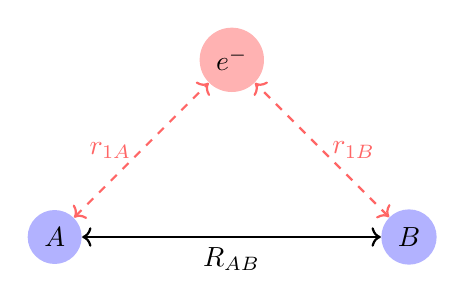
\begin{tikzpicture}[scale=1.5]
\node[circle,fill=blue!30,minimum size=0.6cm] (A) at (0,0) {$A$};
\node[circle,fill=blue!30,minimum size=0.6cm] (B) at (3,0) {$B$};
\node[circle,fill=red!30,minimum size=0.4cm] (e) at (1.5,1.5) {$e^-$};
\draw[<->,thick] (A) -- node[below] {$R_{AB}$} (B);
\draw[<->,thick,dashed,red!60] (A) -- node[left] {$r_{1A}$} (e);
\draw[<->,thick,dashed,red!60] (B) -- node[right] {$r_{1B}$} (e);
\end{tikzpicture}
\small
\vspace{0.5em}

\textit{From your homework 2, Problem 1!}
\end{column}
\end{columns}
\end{frame}

\begin{frame}{The Born--Oppenheimer Approximation}
\begin{block}{Key Idea}
Nuclei are $\sim$1836$\times$ heavier than electrons $\Rightarrow$ electrons respond \emphr{instantaneously} to nuclear motion.
\end{block}

\vspace{0.5em}
\textbf{Separation of variables:}
\[
\Psi_\text{total}(\mathbf{r}, \mathbf{R}) \approx \psi_\text{elec}(\mathbf{r}; \mathbf{R}) \cdot \chi_\text{nuc}(\mathbf{R})
\]

\begin{enumerate}
\item \textbf{Fix} the nuclear positions $\mathbf{R}$ (they become parameters, not variables)
\item \textbf{Solve} the electronic Schr\"{o}dinger equation:
\[
\hat{H}_\text{elec}\,\psi_\text{elec}(\mathbf{r};\mathbf{R}) = E_\text{elec}(\mathbf{R})\,\psi_\text{elec}(\mathbf{r};\mathbf{R})
\]
\item The electronic energy $E_\text{elec}(\mathbf{R})$ \emphr{depends on nuclear positions} $\rightarrow$ this creates the \textbf{Potential Energy Surface (PES)}
\item Nuclei move on this PES
\end{enumerate}
\end{frame}

\begin{frame}{The Electronic Hamiltonian}
After the Born--Oppenheimer approximation, we solve:
\[
\hat{H}_\text{elec} = -\frac{1}{2}\sum_{i=1}^{N}\nabla_i^2 - \sum_{i=1}^{N}\sum_{A=1}^{M}\frac{Z_A}{r_{iA}} + \sum_{i>j}^{N}\frac{1}{r_{ij}}
\]

\vspace{0.5em}
\begin{itemize}
\item Nuclear--nuclear repulsion $V_{nn} = \sum_{A>B}\frac{Z_AZ_B}{R_{AB}}$ is just a \emphr{constant} for fixed $\mathbf{R}$
\item The total energy at a given geometry is:
\[
E_\text{total}(\mathbf{R}) = E_\text{elec}(\mathbf{R}) + V_{nn}(\mathbf{R})
\]
\end{itemize}

\vspace{0.5em}
\begin{tcolorbox}[colback=blue!5!white,colframe=blue!50!black,title=The Electronic Structure Problem]
Given: nuclear positions $\mathbf{R}$ and number of electrons $N$\\
Find: $E_\text{elec}(\mathbf{R})$ and $\psi_\text{elec}(\mathbf{r};\mathbf{R})$\\
\textbf{This is what DFT (and HF, MP2, CC, ...) solves!}
\end{tcolorbox}
\end{frame}


% ============================================================================
% SECTION 3: ELECTRONIC STRUCTURE METHODS
% ============================================================================
\section{Electronic Structure Methods}

\begin{frame}{Approach 1: Wavefunction-Based Methods}
\textbf{Idea:} Approximate the many-electron wavefunction $\Psi(\mathbf{r}_1, \mathbf{r}_2, \ldots, \mathbf{r}_N)$ directly.

\vspace{0.5em}
\textbf{Hartree--Fock (HF) Theory:}
\begin{itemize}
\item Approximate $\Psi$ as a single \textbf{Slater determinant} (antisymmetrized product of one-electron orbitals):
\[
\Psi_\text{HF} = \frac{1}{\sqrt{N!}} \begin{vmatrix} \phi_1(\mathbf{r}_1) & \phi_2(\mathbf{r}_1) & \cdots & \phi_N(\mathbf{r}_1) \\ \phi_1(\mathbf{r}_2) & \phi_2(\mathbf{r}_2) & \cdots & \phi_N(\mathbf{r}_2) \\ \vdots & \vdots & \ddots & \vdots \\ \phi_1(\mathbf{r}_N) & \phi_2(\mathbf{r}_N) & \cdots & \phi_N(\mathbf{r}_N) \end{vmatrix}
\]
\item Automatically satisfies the \textbf{Pauli exclusion principle} (antisymmetry)
\item Each electron moves in the \emphr{average field} of all other electrons
\end{itemize}
\end{frame}

\begin{frame}{Hartree--Fock Energy Expression}
The HF energy is obtained by minimizing $\braket{\Psi_\text{HF}|\hat{H}|\Psi_\text{HF}}$:
\[
E_\text{HF} = \sum_i h_i + \frac{1}{2}\sum_{ij}\left(J_{ij} - K_{ij}\right)
\]

\begin{columns}
\begin{column}{0.48\textwidth}
\begin{itemize}
\item $h_i$ = one-electron integrals\\
{\small (kinetic energy + nuclear attraction)}
\item $J_{ij}$ = \textbf{Coulomb integrals}\\
{\small (classical electron--electron repulsion)}
\end{itemize}
\end{column}
\begin{column}{0.48\textwidth}
\begin{itemize}
\item $K_{ij}$ = \textbf{Exchange integrals}\\
{\small (quantum mechanical, no classical analogue)}
\item \emphr{Missing:} electron \textbf{correlation}\\
{\small (electrons avoid each other beyond mean-field)}
\end{itemize}
\end{column}
\end{columns}

\vspace{1em}
\begin{tcolorbox}[colback=red!5!white,colframe=red!50!black]
\textbf{Correlation energy:} $E_\text{corr} = E_\text{exact} - E_\text{HF}$\\
Typically small ($\sim$1\% of total energy) but \emphr{chemically crucial} ($\sim$1 kcal/mol = make or break for chemistry!)
\end{tcolorbox}
\end{frame}

\begin{frame}{What is Exchange?}
\textbf{Exchange} is a purely \emphr{quantum mechanical} effect arising from the antisymmetry of the wavefunction (Pauli exclusion principle).

\vspace{0.5em}
\begin{columns}
\begin{column}{0.55\textwidth}
\textbf{Physical picture:}
\begin{itemize}
\item Two electrons with the \emphr{same spin} cannot be at the same point in space
\item This creates an ``exchange hole'' -- a region of depleted probability around each electron
\item Electrons with parallel spins are kept apart $\Rightarrow$ their repulsion is \emphr{reduced}
\end{itemize}

\vspace{0.5em}
\textbf{In the HF energy:}
\[
K_{ij} = \iint \frac{\phi_i^*(\mathbf{r}_1)\phi_j(\mathbf{r}_1)\,\phi_j^*(\mathbf{r}_2)\phi_i(\mathbf{r}_2)}{|\mathbf{r}_1 - \mathbf{r}_2|}\,d\mathbf{r}_1\,d\mathbf{r}_2
\]
\begin{itemize}
\item $K_{ij} > 0$ always $\Rightarrow$ exchange \emphr{lowers} the energy ($-K_{ij}$ in $E_\text{HF}$)
\item Non-zero only for same-spin electron pairs
\item No classical analogue -- purely quantum!
\end{itemize}
\end{column}
\begin{column}{0.42\textwidth}
\centering
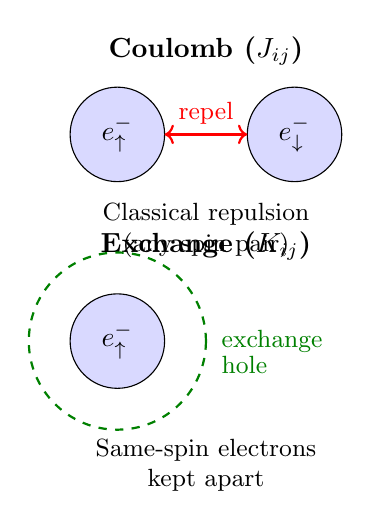
\begin{tikzpicture}[scale=0.75]
% Coulomb - classical picture
\node[above] at (2.5,4.5) {\textbf{Coulomb ($J_{ij}$)}};
\draw[fill=blue!15] (1,3.5) circle (0.8);
\draw[fill=blue!15] (4,3.5) circle (0.8);
\node at (1,3.5) {$e^-_\uparrow$};
\node at (4,3.5) {$e^-_\downarrow$};
\draw[<->,thick,red] (1.8,3.5) -- node[above]{\small repel} (3.2,3.5);
\node[below] at (2.5,2.5) {\small Classical repulsion};
\node[below] at (2.5,2.0) {\small (any spin pair)};
% Exchange - quantum picture
\node[above] at (2.5,1.2) {\textbf{Exchange ($K_{ij}$)}};
\draw[fill=blue!15] (1,0) circle (0.8);
\node at (1,0) {$e^-_\uparrow$};
\draw[dashed,thick,green!50!black] (1,0) circle (1.5);
\node[green!50!black,right] at (2.6,0) {\small exchange};
\node[green!50!black,right] at (2.6,-0.4) {\small hole};
\node[below] at (2.5,-1.5) {\small Same-spin electrons};
\node[below] at (2.5,-2.0) {\small kept apart};
\end{tikzpicture}
\end{column}
\end{columns}
\end{frame}

\begin{frame}{What is Electron Correlation?}
\textbf{Correlation} is everything that HF \emphr{misses} about electron--electron interactions.

\vspace{0.5em}
\begin{columns}
\begin{column}{0.55\textwidth}
\textbf{The HF approximation:}
\begin{itemize}
\item Each electron moves in the \emphr{average} field of all others
\item Electrons don't ``see'' each other's instantaneous positions
\item Like driving on a highway knowing only the \emph{average} traffic density, not where each car actually is
\end{itemize}

\vspace{0.5em}
\textbf{Reality:}
\begin{itemize}
\item Electrons \emphr{avoid each other} dynamically (they are correlated)
\item This creates a ``Coulomb hole'' around each electron
\item Correlation \emphr{always lowers} the energy: $E_\text{corr} < 0$
\end{itemize}
\end{column}
\begin{column}{0.42\textwidth}
\begin{tcolorbox}[colback=red!5!white,colframe=red!50!black,title=Types of Correlation]
\textbf{Dynamic correlation:}\\
{\small Short-range avoidance of electrons. Smooth, small effect per pair, but adds up. Captured by MP2, CCSD.}

\vspace{0.3em}
\textbf{Static (non-dynamic):}\\
{\small Near-degeneracy effects. Multiple configurations contribute equally. Needs multi-reference methods (CASSCF).}
\end{tcolorbox}

\vspace{0.5em}
\small \textbf{Key numbers:}\\
$E_\text{corr}(\ch{H2O}) \approx -0.37$ $E_h$\\
$\approx$ 1\% of total energy\\
$\approx$ 230 kcal/mol!
\end{column}
\end{columns}
\end{frame}

\begin{frame}{The Electron Correlation Problem}
\begin{columns}
\begin{column}{0.55\textwidth}
\textbf{Post-HF methods} recover correlation:
\begin{itemize}
\item \textbf{MP2}: 2nd-order perturbation theory
\item \textbf{CCSD}: coupled cluster singles \& doubles
\item \textbf{CCSD(T)}: ``gold standard'' of quantum chemistry
\item \textbf{Full CI}: exact (within basis set), but scales as $\sim N!$
\end{itemize}

\vspace{0.5em}
\textbf{Problem:} Cost scales steeply with system size!
\begin{itemize}
\item HF: $\mathcal{O}(N^3\text{--}N^4)$
\item MP2: $\mathcal{O}(N^5)$
\item CCSD: $\mathcal{O}(N^6)$
\item CCSD(T): $\mathcal{O}(N^7)$
\end{itemize}
\end{column}
\begin{column}{0.42\textwidth}
\centering

\includegraphics[width=\textwidth]{HF_vs_DFT.png}
\end{column}
\end{columns}
\vspace{0.5em}
\centering
$\Rightarrow$ Need a method that includes correlation at \emphr{lower cost}... \textbf{Enter DFT!}
\end{frame}


% ============================================================================
% SECTION 4: DENSITY FUNCTIONAL THEORY
% ============================================================================
\section{Density Functional Theory}

\begin{frame}{Approach 2: Density Functional Theory}
\begin{columns}
\begin{column}{0.55\textwidth}
\textbf{Key insight:} Instead of the wavefunction $\Psi(\mathbf{r}_1, \ldots, \mathbf{r}_N)$ (depends on $3N$ coordinates), use the \emphr{electron density} $\rho(\mathbf{r})$ (depends on only 3 coordinates!).

\vspace{1em}
\[
\rho(\mathbf{r}) = N \int |\Psi(\mathbf{r}, \mathbf{r}_2, \ldots, \mathbf{r}_N)|^2 \, d\mathbf{r}_2 \cdots d\mathbf{r}_N
\]

\vspace{0.5em}
\begin{itemize}
\item $\rho(\mathbf{r}) \geq 0$ everywhere
\item $\int \rho(\mathbf{r})\,d\mathbf{r} = N$
\item $\rho$ is a \textbf{physical observable} (measurable by X-ray diffraction!)
\end{itemize}
\end{column}
\begin{column}{0.42\textwidth}
\centering
\includegraphics[width=0.9\textwidth]{density_benzene.png}\\
\small Electron density of benzene
\end{column}
\end{columns}
\end{frame}

\begin{frame}{Hohenberg--Kohn Theorems (1964)}
\begin{block}{Theorem 1: Existence}
The ground-state electron density $\rho_0(\mathbf{r})$ \emphr{uniquely determines} the external potential $v_\text{ext}(\mathbf{r})$ (and hence all ground-state properties).
\[
\rho_0(\mathbf{r}) \xrightarrow{\text{1-to-1}} v_\text{ext}(\mathbf{r}) \rightarrow \hat{H} \rightarrow \Psi_0 \rightarrow E_0, \text{all properties}
\]
\end{block}

\begin{block}{Theorem 2: Variational Principle}
The ground-state energy is a \emphr{functional} of the density, and:
\[
E[\rho] \geq E_0 \quad \text{for all trial densities } \rho
\]
The true ground-state density minimizes the energy functional.
\end{block}

\vspace{0.5em}
\textbf{Great news:} Everything is determined by $\rho(\mathbf{r})$.\\
\textbf{Bad news:} We don't know the exact form of $E[\rho]$!
\end{frame}

\begin{frame}{Kohn--Sham DFT (1965)}
\textbf{Kohn \& Sham's brilliant idea:} Introduce a \emphr{fictitious non-interacting system} with the same density as the real one.

\vspace{0.5em}
The Kohn--Sham energy functional:
\[
E_\text{KS}[\rho] = \underbrace{T_s[\rho]}_{\text{KS kinetic}} + \underbrace{\int v_\text{ext}(\mathbf{r})\rho(\mathbf{r})\,d\mathbf{r}}_{E_\text{ext}} + \underbrace{\frac{1}{2}\iint \frac{\rho(\mathbf{r})\rho(\mathbf{r}')}{|\mathbf{r}-\mathbf{r}'|}\,d\mathbf{r}\,d\mathbf{r}'}_{J[\rho] \text{ (Coulomb)}} + \underbrace{E_\text{XC}[\rho]}_{\text{exchange-correlation}}
\]

\vspace{0.5em}
\begin{itemize}
\item $T_s[\rho]$: kinetic energy of \emphr{non-interacting} KS electrons (exact for KS orbitals)
\item $J[\rho]$: classical Coulomb repulsion
\item $E_\text{XC}[\rho]$: \emphr{everything else} -- exchange, correlation, correction to $T_s$
\end{itemize}

\vspace{0.5em}
\begin{tcolorbox}[colback=green!5!white,colframe=green!50!black]
\textbf{The XC functional} $E_\text{XC}[\rho]$ \textbf{is the only unknown!}\\
All of DFT development is about finding better approximations to $E_\text{XC}$.
\end{tcolorbox}
\end{frame}

\begin{frame}{The Kohn--Sham Equations}
Minimizing $E_\text{KS}[\rho]$ leads to one-electron equations:
\[
\left[-\frac{1}{2}\nabla^2 + v_\text{eff}(\mathbf{r})\right]\phi_i(\mathbf{r}) = \varepsilon_i \phi_i(\mathbf{r})
\]
where the effective potential is:
\[
v_\text{eff}(\mathbf{r}) = v_\text{ext}(\mathbf{r}) + \int\frac{\rho(\mathbf{r}')}{|\mathbf{r}-\mathbf{r}'|}d\mathbf{r}' + v_\text{XC}(\mathbf{r})
\]

\vspace{0.5em}
\textbf{Self-Consistent Field (SCF) procedure:}
\begin{enumerate}
\item Guess initial density $\rho^{(0)}(\mathbf{r})$
\item Construct $v_\text{eff}$ from current $\rho$
\item Solve KS equations $\rightarrow$ get orbitals $\{\phi_i\}$
\item Compute new density: $\rho^{(n+1)}(\mathbf{r}) = \sum_{i=1}^{N}|\phi_i(\mathbf{r})|^2$
\item If converged, stop. Otherwise, go to step 2.
\end{enumerate}
\end{frame}

\begin{frame}{HF vs.\ DFT -- A Comparison}
\begin{center}
\begin{tabular}{lcc}
\toprule
& \textbf{Hartree--Fock} & \textbf{Kohn--Sham DFT} \\
\midrule
Central quantity & Wavefunction $\Psi$ & Density $\rho(\mathbf{r})$ \\
Equations & HF equations & KS equations \\
Exchange & Exact (from $\Psi$) & Approximated in $E_\text{XC}$ \\
Correlation & \emphr{Missing} & Included in $E_\text{XC}$ \\
Cost & $\mathcal{O}(N^3\text{--}N^4)$ & $\mathcal{O}(N^3)$ \\
Systematic improvement & Yes (MP2, CC, ...) & \emphr{No} (no ``Jacob's ladder'' guarantee) \\
\bottomrule
\end{tabular}
\end{center}

\vspace{1em}
\textbf{DFT advantage:} Includes correlation at nearly the same cost as HF!\\
\textbf{DFT disadvantage:} The exact $E_\text{XC}$ is unknown -- results depend on the chosen functional.
\end{frame}

\begin{frame}{Jacob's Ladder of Density Functional Approximations}
\begin{columns}
\begin{column}{0.50\textwidth}
\centering

\includegraphics[width=\textwidth]{DFAs.png}
\end{column}
\begin{column}{0.48\textwidth}
\textbf{Perdew's ``Jacob's Ladder''} -- increasing accuracy (and cost):

\vspace{0.5em}
\begin{enumerate}
\item \textbf{LDA}: $E_\text{XC}[\rho]$\\
{\small Local density only; uniform electron gas}
\item \textbf{GGA}: $E_\text{XC}[\rho, \nabla\rho]$\\
{\small PBE, BLYP -- includes density gradient}
\item \textbf{meta-GGA}: $E_\text{XC}[\rho, \nabla\rho, \tau]$\\
{\small TPSS, SCAN -- adds kinetic energy density}
\item \textbf{Hybrid}: mix in exact (HF) exchange\\
{\small B3LYP, PBE0 -- the workhorses of chemistry!}
\item \textbf{Double hybrid}: + MP2 correlation\\
{\small Most accurate, most expensive}
\end{enumerate}
\end{column}
\end{columns}
\end{frame}

\begin{frame}{Common Functionals in Chemistry}
\begin{center}
\begin{tabular}{llcc}
\toprule
\textbf{Functional} & \textbf{Rung} & \textbf{HF Exchange} & \textbf{Common Use} \\
\midrule
LDA (SVWN) & 1 & 0\% & Solids (outdated for molecules) \\
PBE & 2 (GGA) & 0\% & Solids, surfaces \\
BLYP & 2 (GGA) & 0\% & Organic chemistry \\
B3LYP & 4 (Hybrid) & 20\% & \emphr{Most popular in chemistry} \\
PBE0 & 4 (Hybrid) & 25\% & General purpose \\
$\omega$B97X-D & 4 (RSH) & varies & NCI, thermo \\
B2PLYP & 5 (DH) & 53\% & High accuracy \\
\bottomrule
\end{tabular}
\end{center}

\vspace{0.5em}
\textbf{Rules of thumb:}
\begin{itemize}
\item For organic reactions: \textbf{B3LYP-D3} or \textbf{$\omega$B97X-D} with a triple-$\zeta$ basis set
\item For transition metals: \textbf{PBE0} or \textbf{TPSSh}
\item Always consider \emphr{dispersion corrections} (D3, D4, XDM) for non-covalent interactions!
\end{itemize}
\end{frame}

\begin{frame}{Basis Sets -- Expanding the Orbitals}
KS orbitals $\phi_i(\mathbf{r})$ are expanded in a \textbf{basis set}:
\[
\phi_i(\mathbf{r}) = \sum_{\mu} c_{\mu i}\,\chi_\mu(\mathbf{r})
\]
where $\chi_\mu$ are basis functions centered on atoms (usually Gaussians).

\vspace{0.5em}
\textbf{Common naming:} Pople or Dunning basis sets
\begin{itemize}
\item \textbf{STO-3G}: minimal (1 function per orbital) -- \emphr{too small for production}
\item \textbf{6-31G(d)}: split-valence + polarization -- okay for quick checks
\item \textbf{6-311+G(d,p)}: triple-$\zeta$ + diffuse + polarization
\item \textbf{cc-pVDZ, cc-pVTZ, cc-pVQZ}: correlation-consistent, systematically improvable
\item \textbf{def2-TZVP}: efficient, well-balanced for DFT
\end{itemize}

\vspace{0.5em}
\textbf{Rule:} At minimum a \textbf{triple-$\zeta$} basis with \textbf{polarization} for reliable results.\\
Larger basis $\rightarrow$ better results, but more expensive.
\end{frame}

\begin{frame}{Decoding Basis Set Names}
\textbf{Example:} What does \textbf{6-311+G(d,p)} actually mean?

\vspace{0.5em}
\begin{itemize}
\item \textbf{6}: Core orbitals use a contraction of 6 primitive Gaussians
\item \textbf{311}: Valence orbitals split into \emphr{three} sets (triple-$\zeta$)
\begin{itemize}
\item 3 primitives (tight), 1 primitive (medium), 1 primitive (diffuse)
\end{itemize}
\item \textbf{G}: Gaussian-type orbitals (not Slater-type)
\item \textbf{+}: Diffuse functions on heavy atoms (for anions, weak interactions)
\item \textbf{(d,p)}: Polarization functions --- $d$ on heavy atoms, $p$ on H
\end{itemize}

\vspace{0.5em}
\textbf{Other common families:}
\begin{center}
\begin{tabular}{ll}
\toprule
\textbf{Name} & \textbf{Description} \\
\midrule
cc-pVDZ / cc-pVTZ / cc-pVQZ & Correlation-consistent: DZ, TZ, QZ \\
aug-cc-pVTZ & + diffuse functions (for anions, weak interactions) \\
def2-SVP / def2-TZVP & Karlsruhe: efficient, well-balanced for DFT \\
\bottomrule
\end{tabular}
\end{center}
\end{frame}

\begin{frame}{DFT Workflow in Practice}
\begin{center}
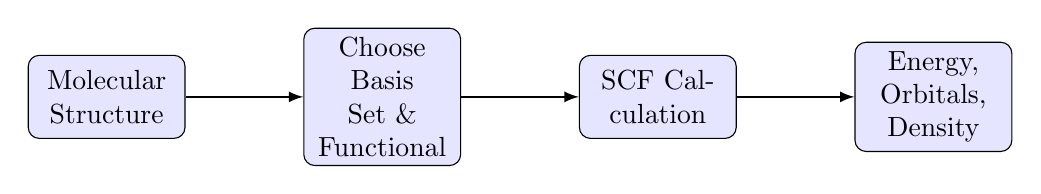
\begin{tikzpicture}[node distance=1.5cm, auto,
    block/.style={rectangle, draw, fill=blue!10, text width=5em, text centered, rounded corners, minimum height=3em},
    line/.style={draw, -latex, thick}]

    \node [block] (input) {Molecular Structure};
    \node [block, right of=input, node distance=3.5cm] (basis) {Choose Basis Set \& Functional};
    \node [block, right of=basis, node distance=3.5cm] (scf) {SCF Calculation};
    \node [block, right of=scf, node distance=3.5cm] (output) {Energy, Orbitals, Density};

    \path [line] (input) -- (basis);
    \path [line] (basis) -- (scf);
    \path [line] (scf) -- (output);
\end{tikzpicture}
\end{center}

\vspace{1em}
\textbf{Input requires:}
\begin{itemize}
\item Atomic coordinates (Cartesian or Z-matrix)
\item Charge and spin multiplicity
\item Choice of method (functional) and basis set
\item Type of calculation (energy, optimization, frequency, ...)
\end{itemize}

\vspace{0.5em}
\textbf{Software:} Gaussian, ORCA, Q-Chem, Psi4, FHI-aims, Quantum ESPRESSO, ...
\end{frame}


% ============================================================================
% SECTION 5: THE POTENTIAL ENERGY SURFACE
% ============================================================================
\section{The Potential Energy Surface}

\begin{frame}{The Potential Energy Surface (PES)}
\begin{columns}
\begin{column}{0.50\textwidth}
\centering
\includegraphics[width=\textwidth]{PES.png}
\end{column}
\begin{column}{0.48\textwidth}
$E_\text{total}(\mathbf{R})$ as a function of all nuclear coordinates defines the \textbf{PES}.

\vspace{0.5em}
For $M$ atoms: PES has $3M - 6$ dimensions ($3M-5$ for linear).

\vspace{0.5em}
\textbf{Key features:}
\begin{itemize}
\item \textbf{Minima}: stable structures (reactants, products, intermediates)
\item \textbf{Saddle points}: transition states
\item \textbf{Gradient} $= \nabla E$: forces on atoms
\item \textbf{Hessian} $= \nabla^2 E$: curvature (force constants)
\end{itemize}
\end{column}
\end{columns}
\end{frame}

\begin{frame}{Types of Calculations on the PES}
\begin{columns}
\begin{column}{0.32\textwidth}
\centering

\includegraphics[height=0.35\textheight]{single_point.png}\\
\textbf{Single-Point Energy}\\
\small
Energy at one fixed geometry.\\
$E(\mathbf{R}_0)$
\end{column}
\begin{column}{0.32\textwidth}
\centering

\includegraphics[height=0.35\textheight]{geom_opt.png}\\
\textbf{Geometry Optimization}\\
\small
Follow gradient downhill to find minimum.\\
$\nabla E = \mathbf{0}$
\end{column}
\begin{column}{0.32\textwidth}
\centering
\includegraphics[height=0.35\textheight]{Frequencies.png}\\
\textbf{Frequency Calculation}\\
\small
Compute Hessian $\rightarrow$ normal modes.\\
Verify min.\ or TS.
\end{column}
\end{columns}

\vspace{1em}
\begin{tcolorbox}[colback=blue!5!white,colframe=blue!50!black]
\textbf{At a minimum:} all frequencies real (positive eigenvalues of Hessian)\\
\textbf{At a transition state:} exactly \emphr{one imaginary frequency} (one negative eigenvalue)
\end{tcolorbox}
\end{frame}

\begin{frame}{Geometry Optimization -- Finding Minima}
\textbf{Algorithm:} Follow the forces (negative gradient) downhill:

\vspace{0.5em}
\begin{enumerate}
\item Start with initial geometry $\mathbf{R}_0$
\item Compute energy $E(\mathbf{R}_0)$ and gradient $\mathbf{g}_0 = \nabla E|_{\mathbf{R}_0}$
\item Take a step: $\mathbf{R}_1 = \mathbf{R}_0 - \alpha \, \mathbf{g}_0$ \quad (steepest descent)
\item Repeat until $|\mathbf{g}| < \text{threshold}$ and $|\Delta E| < \text{threshold}$
\end{enumerate}

\vspace{0.5em}
\textbf{Better algorithms:} Newton--Raphson uses Hessian information:
\[
\mathbf{R}_{n+1} = \mathbf{R}_n - \mathbf{H}^{-1}\,\mathbf{g}_n
\]

\vspace{0.5em}
\textbf{Convergence criteria} (typical):
\begin{itemize}
\item Max force $< 4.5 \times 10^{-4}$ hartree/bohr
\item RMS force $< 3.0 \times 10^{-4}$ hartree/bohr
\item Max displacement $< 1.8 \times 10^{-3}$ bohr
\item RMS displacement $< 1.2 \times 10^{-3}$ bohr
\end{itemize}
\end{frame}


% ============================================================================
% SECTION 6: HARMONIC APPROXIMATION
% ============================================================================
\section{The Harmonic Approximation}

\begin{frame}{Beyond Electronic Energy -- We Need Vibrations!}
\textbf{DFT gives us} $E_\text{elec}(\mathbf{R})$ -- but thermodynamics requires knowledge of \emphr{nuclear motion}.

\vspace{0.5em}
\textbf{The bridge:}
\[
E_\text{elec}(\mathbf{R}) \xrightarrow{\text{harmonic approx.}} \text{frequencies } \{\nu_k\} \xrightarrow{\text{stat.\ mech.}} q_\text{vib} \xrightarrow{} \Delta G, \Delta H, \Delta S, K_\text{eq}, k(T)
\]

\vspace{1em}
\begin{tcolorbox}[colback=green!5!white,colframe=green!50!black,title=The Key Connection]
\centering
The harmonic approximation is the \emphr{bridge} between\\
\textbf{quantum chemistry} (electronic structure)\\
and\\
\textbf{statistical thermodynamics} (macroscopic properties)
\end{tcolorbox}
\end{frame}

\begin{frame}{The Morse Potential and Taylor Expansion}
\begin{columns}
\begin{column}{0.52\textwidth}
\textbf{True potential} for a diatomic (Morse):
\[
V(r) = D_e\left(1 - \e^{-a(r-r_e)}\right)^2
\]

\textbf{Taylor expand} around equilibrium $r_e$:
\[
V(r) \approx \cancelto{V_0}{V(r_e)} + \cancelto{0}{\frac{dV}{dr}\bigg|_{r_e}}\!(r\!-\!r_e) + \frac{1}{2}\underbrace{\frac{d^2V}{dr^2}\bigg|_{r_e}}_{k}(r\!-\!r_e)^2 + \cdots
\]

$\Rightarrow$ Near equilibrium: $\boxed{V(r) \approx \tfrac{1}{2}k(r-r_e)^2}$

\vspace{0.3em}
\begin{itemize}
\item $k = \frac{d^2V}{dr^2}\big|_{r_e}$ is the \textbf{force constant}
\item Harmonic approx.\ valid near minimum
\item Breaks down far from $r_e$ (dissociation)
\end{itemize}

\vspace{0.3em}
\small\textit{From your homework 2, Problem 2!}
\end{column}
\begin{column}{0.45\textwidth}
\centering

\includegraphics[width=\textwidth]{harmonic.png}

\small Comparison of harmonic (parabolic) approximation with the ``exact'' (Morse-like) potential.
\end{column}
\end{columns}
\end{frame}

\begin{frame}{Force Constants and the Hessian Matrix}
For a \textbf{polyatomic molecule}, the Taylor expansion generalizes to:

\[
V(\mathbf{R}) \approx V(\mathbf{R}_e) + \frac{1}{2}\sum_{i,j} \underbrace{\frac{\partial^2 V}{\partial R_i \partial R_j}\bigg|_{\mathbf{R}_e}}_{H_{ij}} \Delta R_i \,\Delta R_j
\]

\vspace{0.5em}
\begin{tcolorbox}[colback=blue!5!white,colframe=blue!50!black,title=The Hessian Matrix]
\[
\mathbf{H} = \begin{pmatrix}
\frac{\partial^2 V}{\partial R_1^2} & \frac{\partial^2 V}{\partial R_1 \partial R_2} & \cdots \\[6pt]
\frac{\partial^2 V}{\partial R_2 \partial R_1} & \frac{\partial^2 V}{\partial R_2^2} & \cdots \\[6pt]
\vdots & \vdots & \ddots
\end{pmatrix}
\]
The Hessian is a $3M \times 3M$ matrix of second derivatives of the energy with respect to nuclear displacements.\\
\small\textit{Note: In your Week 4 lectures, Anatole called this $\mathbf{M}$. Same matrix, different letter!}
\end{tcolorbox}
\end{frame}

\begin{frame}{Mass-Weighted Coordinates and Normal Modes}
\textbf{Problem:} Cartesian displacements couple different atoms.

\textbf{Solution:} Transform to \emphr{mass-weighted coordinates} (exactly as in Week 4):
\[
q_i = \sqrt{m_i}\,\Delta R_i
\]

The mass-weighted Hessian is:
\[
\tilde{H}_{ij} = \frac{H_{ij}}{\sqrt{m_i m_j}} = \frac{1}{\sqrt{m_i m_j}}\frac{\partial^2 V}{\partial R_i \partial R_j}
\]

\textbf{Diagonalize} $\tilde{\mathbf{H}}$:
\[
\tilde{\mathbf{H}}\,\mathbf{L} = \mathbf{L}\,\bs{\Lambda}
\]

\begin{itemize}
\item \textbf{Eigenvalues} $\lambda_k$: related to vibrational frequencies $\nu_k = \frac{1}{2\pi}\sqrt{\lambda_k}$
\item \textbf{Eigenvectors}: the \emphr{normal modes} -- independent vibrational motions
\item 6 eigenvalues $= 0$ (translations + rotations); $3M-6$ are vibrational
\end{itemize}
\end{frame}

\begin{frame}{Normal Modes -- Physical Meaning}
\begin{columns}
\begin{column}{0.55\textwidth}
\textbf{Normal modes} are \emphr{independent} vibrations where all atoms move in phase at the same frequency.

\vspace{0.5em}
\textbf{Example: Linear triatomic} (\ch{CO2}):
\begin{itemize}
\item $3(3) - 5 = 4$ vibrational modes
\item Symmetric stretch: $\nu_1 = 1388$ cm$^{-1}$
\item Asymmetric stretch: $\nu_3 = 2349$ cm$^{-1}$
\item Bending (2$\times$ degenerate): $\nu_2 = 667$ cm$^{-1}$
\end{itemize}

\vspace{0.5em}
\small\textit{From your homework 2, Problem 3!}\\
\small You diagonalized the Hessian for a linear triatomic to find these modes.
\end{column}
\begin{column}{0.42\textwidth}
\centering
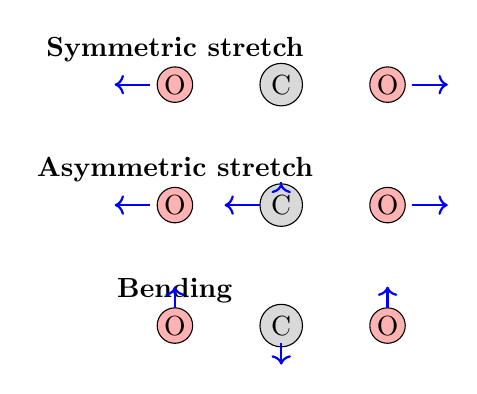
\begin{tikzpicture}[scale=0.9]
% Symmetric stretch
\node at (0,3.5) {\textbf{Symmetric stretch}};
\draw[fill=red!30] (0,3) circle (0.25) node {O};
\draw[fill=gray!30] (1.5,3) circle (0.3) node {C};
\draw[fill=red!30] (3,3) circle (0.25) node {O};
\draw[->,thick,blue] (-0.35,3) -- (-0.85,3);
\draw[->,thick,blue] (3.35,3) -- (3.85,3);
% Asymmetric stretch
\node at (0,1.8) {\textbf{Asymmetric stretch}};
\draw[fill=red!30] (0,1.3) circle (0.25) node {O};
\draw[fill=gray!30] (1.5,1.3) circle (0.3) node {C};
\draw[fill=red!30] (3,1.3) circle (0.25) node {O};
\draw[->,thick,blue] (-0.35,1.3) -- (-0.85,1.3);
\draw[->,thick,blue] (1.5,1.6) -- (1.5,1.6);
\draw[->,thick,blue] (3.35,1.3) -- (3.85,1.3);
\draw[->,thick,blue] (1.2,1.3) -- (0.7,1.3);
% Bending
\node at (0,0.1) {\textbf{Bending}};
\draw[fill=red!30] (0,-0.4) circle (0.25) node {O};
\draw[fill=gray!30] (1.5,-0.4) circle (0.3) node {C};
\draw[fill=red!30] (3,-0.4) circle (0.25) node {O};
\draw[->,thick,blue] (0,-0.15) -- (0,0.15);
\draw[->,thick,blue] (1.5,-0.65) -- (1.5,-0.95);
\draw[->,thick,blue] (3,-0.15) -- (3,0.15);
\end{tikzpicture}
\end{column}
\end{columns}
\end{frame}

\begin{frame}{The Harmonic Oscillator -- Quantum Energy Levels}
Each normal mode $k$ behaves as an independent \textbf{quantum harmonic oscillator}:

\[
\varepsilon_{k,n} = \left(n + \frac{1}{2}\right)h\nu_k = \left(n + \frac{1}{2}\right)\hbar\omega_k, \qquad n = 0, 1, 2, \ldots
\]

\small\textit{You derived $E = \hbar\omega(n+\tfrac{1}{2})$ in Week 4. Same result --- $h\nu = \hbar\omega$ since $\omega = 2\pi\nu$.}

\vspace{0.3em}
\textbf{Key features:}
\begin{itemize}
\item \textbf{Zero-point energy (ZPE):} Even at $T = 0$ K, $\varepsilon_{k,0} = \frac{1}{2}h\nu_k \neq 0$
\item Total ZPE: $E_\text{ZPE} = \frac{1}{2}\sum_{k=1}^{3M-6} h\nu_k$
\item Equally spaced energy levels (spacing $= h\nu_k$)
\item Good approximation near the bottom of the potential well
\end{itemize}

\vspace{0.5em}
\begin{tcolorbox}[colback=yellow!5!white,colframe=yellow!50!black]
\textbf{Important:} The \emphr{zero-point energy} is a quantum effect with no classical analogue. It affects reaction energies and must always be included!
\end{tcolorbox}
\end{frame}


% ============================================================================
% SECTION 7: PARTITION FUNCTIONS FROM DFT
% ============================================================================
\section{Partition Functions from DFT}

\begin{frame}{Statistical Mechanics Recap}
\textbf{Connection:} Microscopic energy levels $\rightarrow$ macroscopic thermodynamics

\vspace{0.5em}
\textbf{Canonical partition function} (using $\beta = 1/k_BT$ as in your lectures):
\[
Q(N,V,T) = \sum_j \e^{-\beta E_j} = \sum_j \e^{-E_j / k_B T}
\]

For $N$ \emphr{indistinguishable, independent} molecules:
\[
Q = \frac{q^N}{N!}
\]
where $q$ is the \textbf{molecular partition function}.

\vspace{0.5em}
\textbf{Key thermodynamic relations} (you've derived these since Week 6):
\begin{align*}
A &= -k_B T \ln Q & \text{(Helmholtz free energy)} \\
U &= \langle E \rangle = -\frac{\partial \ln Q}{\partial \beta} = k_B T^2 \left(\frac{\partial \ln Q}{\partial T}\right)_{N,V} & \text{(internal energy)} \\
S &= k_B\,\partial_T(T \ln Q) & \text{(entropy)}
\end{align*}
\end{frame}

\begin{frame}{Factorization of the Molecular Partition Function}
Within the Born--Oppenheimer and rigid-rotor/harmonic-oscillator (RRHO) approximations:

\[
\boxed{q = q_\text{trans} \cdot q_\text{rot} \cdot q_\text{vib} \cdot q_\text{elec}}
\]

\vspace{0.5em}
Each factor corresponds to an \emphr{independent} degree of freedom:

\begin{center}
\begin{tabular}{lll}
\toprule
\textbf{Factor} & \textbf{Information from DFT} & \textbf{Depends on} \\
\midrule
$q_\text{trans}$ & Molecular mass & $T$, $V$ (or $P$) \\
$q_\text{rot}$ & Moments of inertia (from optimized geometry) & $T$ \\
$q_\text{vib}$ & Vibrational frequencies (from Hessian) & $T$ \\
$q_\text{elec}$ & Electronic energy, degeneracy & $T$ (usually $\approx 1$) \\
\bottomrule
\end{tabular}
\end{center}

\vspace{0.5em}
\textbf{DFT frequency calculation gives us everything we need!}
\end{frame}

\begin{frame}{Translational Partition Function}
\small\textit{You derived this from PIB eigenvalues in Week 6: $q^\text{trans} = (2\pi m / \beta h^2)^{3/2} V$.}

\vspace{0.3em}
For an ideal gas in a box of volume $V$:
\[
q_\text{trans} = \left(\frac{2\pi m k_B T}{h^2}\right)^{3/2} V = \frac{V}{\Lambda^3}
\]

where $\Lambda$ is the \textbf{thermal de Broglie wavelength}:
\[
\Lambda = \frac{h}{\sqrt{2\pi m k_B T}}
\]

\vspace{0.5em}
\begin{itemize}
\item $m$ = total molecular mass (sum of atomic masses)
\item Typically $q_\text{trans} \sim 10^{30}$ at room temperature
\item Dominant contribution to the entropy
\item Often evaluated at standard pressure: $V = k_B T / P^\circ$
\end{itemize}
\end{frame}

\begin{frame}{Rotational Partition Function}
For a \textbf{nonlinear polyatomic} molecule (rigid rotor, high-$T$ limit):
\[
q_\text{rot} = \frac{\sqrt{\pi}}{\sigma} \left(\frac{8\pi^2 k_B T}{h^2}\right)^{3/2} \sqrt{I_A I_B I_C}
\]

\begin{itemize}
\item $I_A, I_B, I_C$ = principal moments of inertia (from optimized geometry)
\item $\sigma$ = \textbf{rotational symmetry number}
\begin{itemize}
\item \ch{H2O}: $\sigma = 2$ \quad (C$_{2v}$)
\item \ch{NH3}: $\sigma = 3$ \quad (C$_{3v}$)
\item \ch{CH4}: $\sigma = 12$ \quad (T$_d$)
\item \ch{C6H6}: $\sigma = 12$ \quad (D$_{6h}$)
\end{itemize}
\item For a \textbf{linear molecule}: $q_\text{rot} = \frac{8\pi^2 I k_B T}{\sigma h^2}$
\end{itemize}
\end{frame}

\begin{frame}{Vibrational Partition Function}
For a \textbf{harmonic oscillator} with frequency $\nu_k$:
\[
q_{\text{vib},k} = \frac{1}{1 - \e^{-h\nu_k / k_BT}} = \frac{1}{1 - \e^{-\Theta_{V,k}/T}}
\]
where $\Theta_{V,k} = h\nu_k / k_B$ is the \textbf{vibrational temperature}.

\vspace{0.5em}
Total vibrational partition function (modes are independent):
\[
q_\text{vib} = \prod_{k=1}^{3M-6} q_{\text{vib},k} = \prod_{k=1}^{3M-6} \frac{1}{1 - \e^{-\Theta_{V,k}/T}}
\]

\vspace{0.5em}
\textbf{Key limits:}
\begin{itemize}
\item $T \ll \Theta_V$: mode is ``frozen'', $q_{\text{vib},k} \approx 1$ (only ground state populated)
\item $T \gg \Theta_V$: classical limit, $q_{\text{vib},k} \approx T/\Theta_V = k_BT/h\nu_k$
\end{itemize}

\vspace{0.5em}
\small \textbf{Example:} C--H stretch $\sim 3000$ cm$^{-1}$ $\Rightarrow$ $\Theta_V \approx 4300$ K (frozen at RT)\\
Low-frequency torsion $\sim 100$ cm$^{-1}$ $\Rightarrow$ $\Theta_V \approx 144$ K (classical at RT)
\end{frame}

\begin{frame}{Vibrational Partition Function -- Including ZPE}
\textbf{Two conventions:}

\vspace{0.5em}
\textbf{Bottom-of-the-well (BOW):}
\[
q_\text{vib}^\text{BOW} = \prod_{k=1}^{3M-6} \frac{\e^{-\Theta_{V,k}/2T}}{1 - \e^{-\Theta_{V,k}/T}}
\]
Energy measured from the minimum of the PES.

\vspace{0.5em}
\textbf{Zero-point exclusive (V=0):}
\[
q_\text{vib}^\text{V=0} = \prod_{k=1}^{3M-6} \frac{1}{1 - \e^{-\Theta_{V,k}/T}}
\]
Energy measured from the ZPE level.

\vspace{0.5em}
\begin{tcolorbox}[colback=yellow!5!white,colframe=yellow!50!black]
Most quantum chemistry programs (Gaussian, ORCA) use the BOW convention and report total energy as: $E_\text{total} = E_\text{elec} + E_\text{ZPE} + E_\text{thermal}$
\end{tcolorbox}
\end{frame}

\begin{frame}{Electronic Partition Function}
\[
q_\text{elec} = \sum_j g_j \,\e^{-\varepsilon_j / k_BT}
\]

For most closed-shell molecules at room temperature:
\begin{itemize}
\item Electronic excitation energies $\gg k_B T$ ($\sim$0.026 eV at 298 K)
\item Only the ground state is populated
\item $q_\text{elec} \approx g_0 = 1$ for singlet ground states
\end{itemize}

\vspace{0.5em}
\textbf{Exceptions:}
\begin{itemize}
\item Open-shell species: $g_0 = 2S+1$ (spin degeneracy)
\item Example: \ch{O2} ($^3\Sigma_g^-$): $g_0 = 3$
\item NO ($^2\Pi$): low-lying excited states contribute at high $T$
\end{itemize}
\end{frame}


% ============================================================================
% SECTION 8: THERMODYNAMIC PROPERTIES FROM DFT
% ============================================================================
\section{Thermodynamic Properties from DFT}

\begin{frame}{Putting It All Together: $G$ from DFT}
\textbf{Total Gibbs free energy} from a DFT frequency calculation:
\[
\boxed{G = E_\text{elec} + E_\text{ZPE} + H_\text{thermal} - TS}
\]

where:
\begin{align*}
E_\text{ZPE} &= \frac{1}{2}\sum_k h\nu_k \\
H_\text{thermal} &= U_\text{trans} + U_\text{rot} + U_\text{vib} + k_BT \\
&= \frac{3}{2}k_BT + \frac{3}{2}k_BT + \sum_k \frac{h\nu_k}{\e^{h\nu_k/k_BT}-1} + k_BT \\
S &= S_\text{trans} + S_\text{rot} + S_\text{vib} + S_\text{elec}
\end{align*}

\vspace{0.5em}
\textbf{Key point:} $E_\text{elec}$ dominates ($\sim$thousands of hartree), but the \emphr{thermal corrections} ($\sim$millihartree) determine \emphr{relative} energies and selectivities!
\end{frame}

\begin{frame}{Entropy Contributions}
\textbf{Translational entropy} (Sackur--Tetrode equation):
\[
S_\text{trans} = R\left[\ln\left(\frac{q_\text{trans}}{N}\right) + \frac{5}{2}\right]
\]

\textbf{Rotational entropy:}
\[
S_\text{rot} = R\left[\ln q_\text{rot} + \frac{3}{2}\right] \quad \text{(nonlinear)}
\]

\textbf{Vibrational entropy:}
\[
S_\text{vib} = R\sum_k \left[\frac{\Theta_{V,k}/T}{\e^{\Theta_{V,k}/T}-1} - \ln\left(1 - \e^{-\Theta_{V,k}/T}\right)\right]
\]

\vspace{0.5em}
\begin{itemize}
\item $S_\text{trans}$ is the \emphr{largest} contribution (typically $\sim$150 J/(mol$\cdot$K))
\item $S_\text{vib}$ matters for low-frequency modes ($\nu < 200$ cm$^{-1}$)
\item At $T \rightarrow 0$: $S \rightarrow 0$ (third law of thermodynamics, $\checkmark$)
\end{itemize}
\end{frame}

\begin{frame}{What a Gaussian/ORCA Output Gives You}
After a \texttt{freq} calculation, you get a thermochemistry summary:

\vspace{0.5em}
\begin{tcolorbox}[colback=snow,colframe=charcoal,fontupper=\ttfamily\scriptsize]
 Zero-point correction=                 0.044749 (Hartree/Particle)\\
 Thermal correction to Energy=          0.047545\\
 Thermal correction to Enthalpy=        0.048489\\
 Thermal correction to Gibbs Free Energy= 0.021178\\
 Sum of electronic and zero-point Energies=   -76.377939\\
 Sum of electronic and thermal Energies=      -76.375143\\
 Sum of electronic and thermal Enthalpies=    -76.374199\\
 Sum of electronic and thermal Free Energies= -76.401510
\end{tcolorbox}

\vspace{0.5em}
\begin{itemize}
\item Use ``Sum of electronic and thermal Free Energies'' for $\Delta G$
\item Compare \emphr{relative} values (products $-$ reactants)
\item Default: $T = 298.15$ K, $P = 1$ atm (can be changed)
\end{itemize}
\end{frame}

\begin{frame}{Computing Reaction Thermodynamics}
\textbf{Example:} Reaction $\ch{A -> B}$

\begin{align*}
\Delta E &= E_\text{elec}(B) - E_\text{elec}(A) & \text{(electronic energy only)} \\
\Delta E_0 &= \Delta E + \Delta E_\text{ZPE} & \text{(ZPE-corrected)} \\
\Delta H &= \Delta E_0 + \Delta H_\text{thermal} & \text{(includes thermal corrections)} \\
\Delta G &= \Delta H - T\Delta S & \text{(includes entropy)}
\end{align*}

\vspace{0.5em}
\begin{tcolorbox}[colback=green!5!white,colframe=green!50!black,title=Hierarchy of Accuracy]
\centering
$\Delta E \neq \Delta E_0 \neq \Delta H \neq \Delta G$\\[6pt]
\small You \emphr{must} include ZPE and thermal corrections for meaningful comparison with experiment!
\end{tcolorbox}

\vspace{0.5em}
\textbf{Equilibrium constant:}
\[
K = \e^{-\Delta G^\circ / RT}
\]
\end{frame}

\begin{frame}{Example: Conformational Energies of Butane}
\begin{columns}
\begin{column}{0.55\textwidth}
\centering
\includegraphics[width=\textwidth]{Butane_conformations_and_relative_energies.png}
\end{column}
\begin{column}{0.42\textwidth}
\textbf{DFT can predict:}
\begin{itemize}
\item Relative energies of conformers
\item Rotational barriers
\item Population ratios via Boltzmann distribution:
\end{itemize}
\[
\frac{N_i}{N_j} = \frac{g_i}{g_j}\e^{-(E_i - E_j)/k_BT}
\]

\vspace{0.5em}
\textbf{At 298 K:}\\
$\Delta G(\text{gauche} - \text{anti})$\\$\approx 0.9$ kcal/mol\\
$\Rightarrow$ $\sim$82\% anti, $\sim$18\% gauche
\end{column}
\end{columns}
\end{frame}


% ============================================================================
% SECTION 9: PRACTICAL CONSIDERATIONS
% ============================================================================
\section{Practical Considerations}

\begin{frame}[fragile]{Reading the Output: From Frequencies to $G$}
\textbf{After a geometry optimization + frequency calculation}, the output file contains everything you need.

\vspace{0.3em}
\textbf{Typical Gaussian output} (near the end of the log file):
\begin{tcolorbox}[colback=snow,colframe=charcoal,fontupper=\ttfamily\scriptsize]
\begin{verbatim}
 Zero-point correction=              0.04489 (Hartree/Particle)
 Thermal correction to Energy=       0.04773
 Thermal correction to Enthalpy=     0.04867
 Thermal correction to Gibbs Free Energy= 0.02236
 Sum of electronic and zero-point Energies=    -76.38295
 Sum of electronic and thermal Energies=       -76.38011
 Sum of electronic and thermal Enthalpies=     -76.37917
 Sum of electronic and thermal Free Energies=  -76.40548
\end{verbatim}
\end{tcolorbox}

\vspace{0.3em}
\textbf{To compute $\Delta G^\circ$ for a reaction:}
\begin{enumerate}
\item Read ``Sum of electronic and thermal Free Energies'' for \emphr{each} species
\item $\Delta G^\circ = \sum G_\text{products} - \sum G_\text{reactants}$
\item $K = \e^{-\Delta G^\circ / RT}$
\end{enumerate}
\small In ORCA: look for ``Final Gibbs free enthalpy'' or ``$G$(298 K)'' in the thermochemistry block.
\end{frame}

\begin{frame}{Limitations of the Harmonic Approximation}
\textbf{The harmonic approximation breaks down for:}
\begin{enumerate}
\item \textbf{Large-amplitude motions:} internal rotations, ring puckering
\begin{itemize}
\item Low frequencies ($< 100$ cm$^{-1}$) are most problematic
\item These contribute significantly to $S_\text{vib}$ and $G$
\end{itemize}
\item \textbf{Anharmonic vibrations:} bond dissociation, highly excited states
\item \textbf{Near-zero frequencies:} flat regions of PES (e.g., methyl rotations)
\end{enumerate}

\vspace{0.5em}
\textbf{Practical fixes:}
\begin{itemize}
\item \textbf{Quasi-harmonic correction} (Truhlar): raise all frequencies $< 100$ cm$^{-1}$ to 100 cm$^{-1}$
\item \textbf{Quasi-RRHO} (Grimme): interpolate between HO and free-rotor models below a cutoff ($\sim$100 cm$^{-1}$)
\item \textbf{ZPE scaling factors:} multiply calculated frequencies by an empirical factor (e.g., 0.9804 for B3LYP/6-31G(d))
\end{itemize}
\end{frame}

\begin{frame}{Summary of Lecture 1}
\begin{enumerate}
\item \textbf{Hamiltonian $\rightarrow$ Born--Oppenheimer:} Separate electronic and nuclear problems
\item \textbf{Electronic structure:} HF treats exchange exactly but misses correlation; DFT includes both via $E_\text{XC}[\rho]$
\item \textbf{Kohn--Sham DFT:} Solve one-electron equations self-consistently; accuracy depends on the chosen functional
\item \textbf{PES:} Energy as a function of nuclear coordinates; minima and saddle points
\item \textbf{Harmonic approximation:} Taylor expansion of PES $\rightarrow$ force constants $\rightarrow$ Hessian $\rightarrow$ normal modes
\item \textbf{Partition functions:} $q = q_\text{trans} \cdot q_\text{rot} \cdot q_\text{vib} \cdot q_\text{elec}$, each computed from DFT output
\item \textbf{Thermodynamics:} $G = E_\text{elec} + E_\text{ZPE} + H_\text{thermal} - TS$
\end{enumerate}

\vspace{1em}
\begin{center}
\textbf{Next lecture:} Transition states, reaction mechanisms, and energy profiles!
\end{center}
\end{frame}

\begin{frame}{Key Equations to Remember}
\begin{columns}
\begin{column}{0.48\textwidth}
\textbf{Electronic Structure:}
\begin{align*}
\hat{H}\Psi &= E\Psi \\
E_\text{KS} &= T_s + E_\text{ext} + J + E_\text{XC} \\
\end{align*}

\textbf{Harmonic Approximation:}
\begin{align*}
V(r) &\approx \tfrac{1}{2}k(r-r_e)^2 \\
\varepsilon_n &= (n+\tfrac{1}{2})h\nu
\end{align*}
\end{column}
\begin{column}{0.48\textwidth}
\textbf{Partition Functions:}
\begin{align*}
q &= q_\text{trans}\cdot q_\text{rot}\cdot q_\text{vib}\cdot q_\text{elec}\\
q_\text{vib} &= \prod_k \frac{1}{1-\e^{-\Theta_{V,k}/T}}
\end{align*}

\textbf{Thermodynamics:}
\begin{align*}
G &= E_\text{elec} + E_\text{ZPE} + H_\text{th} - TS \\
K &= \e^{-\Delta G^\circ/RT}
\end{align*}
\end{column}
\end{columns}
\end{frame}

\end{document}
